% ============================================================ kinetic exchange
\section{Kinetic exchange}

\begin{frame}{The Hubbard picture}
  \begin{paperclaim}
    ``The kinetic exchange picture based on the Hubbard model \dots\ attributes stability of a singlet state in
    the case of orthogonal atomic orbitals (AOs) to the fact that perturbation yielding ionic configuration is
    allowed only from this state, and not from the triplet.'' (p.\ 442)
  \end{paperclaim}
  \vskip0.3cm
  \centering
  \begin{tikzpicture}[scale=1.1]
    \node[circle,draw=noirgold,fill=noirpanel,minimum size=1.0cm,font=\large] (l) at (0,0) {$l$};
    \node[circle,draw=noirgold,fill=noirpanel,minimum size=1.0cm,font=\large] (r) at (4,0) {$r$};
    \onslide<2->{\draw[{Stealth[length=5pt]}-{Stealth[length=5pt]},noircyan,line width=0.9pt] (l) -- node[above,font=\small,text=noircyan]{hopping $h_{lr}=-t$} (r);}
    \onslide<3->{\node[font=\small,text=noirrose] at (0,-0.95) {$U=\eri llll$};\node[font=\small,text=noirrose] at (4,-0.95) {$U=\eri rrrr$};}
    \onslide<4->{\node[font=\small,text=noirviolet] at (2,-0.55) {$V=\eri llrr$};}
    \onslide<5->{\node[font=\small,text=noirgreen] at (2,-1.1) {$k=\eri lrlr\ge0$};}
  \end{tikzpicture}
\end{frame}

\begin{frame}{Step 1: ionic configurations are pure singlets}
  \begin{columns}[c]
    \column{0.55\textwidth}
    \begin{enumerate}
      \item ionic: both electrons in one orbital, $l(1)l(2)$
      \item<2-> that spatial part is \cgold{symmetric}
      \item<3-> antisymmetry $\Rightarrow$ its spin part must be the \cgold{singlet} $\Theta_{0,0}$
      \item<4-> $\Hop$ is spin-free, so
            $\mel{\text{ionic}}{\Hop}{\text{triplet}}\propto\braket{\Theta_{0,0}}{\Theta_{1,M}}=0$
    \end{enumerate}
    \onslide<5->{
    \begin{keyresult}
      only the singlet can borrow from ionic configurations
    \end{keyresult}}
    \column{0.4\textwidth}
    \centering
    \begin{tikzpicture}[scale=1.2]
      \draw[level] (-0.4,0) -- (0.4,0); \draw[level] (0.9,0) -- (1.7,0);
      \elup{0}{0}\eldn{1.3}{0} \node[font=\scriptsize,text=noirmuted] at (0.65,-0.45) {covalent};
      \draw[level] (-0.4,-1.4) -- (0.4,-1.4); \draw[level] (0.9,-1.4) -- (1.7,-1.4);
      \elup{0}{-1.4}\eldn{0}{-1.4} \node[font=\scriptsize,text=noirmuted] at (0.65,-1.85) {ionic $l^2$};
      \onslide<4->{\draw[-{Stealth[length=4pt]},noircyan] (2.0,-0.1) to[bend left=40] node[right,font=\scriptsize]{$-t$} (2.0,-1.3);}
    \end{tikzpicture}
  \end{columns}
\end{frame}

\begin{frame}{Step 2: the matrix}
  insert the parameters into the $2e/2o$ Hamiltonian ($h_{ll}=h_{rr}=0$, $\eri lllr=0$):
  {\large
  \[
    E_T=V-k,\qquad
    \mathbf H_S=\begin{pmatrix}U&k&-\sqrt2t\\k&U&-\sqrt2t\\-\sqrt2t&-\sqrt2t&V+k\end{pmatrix}
    \quad(ll,\ rr,\ \text{cov})
  \]}
  \onslide<2->{\cgold{Step 3}: symmetry-adapt the ionic pair, $\Phi_{\pm}=\tfrac1{\sqrt2}(ll\pm rr)$}
  {\large
  \begin{align*}
    \uncover<3->{E(\Phi_\pm)}&\uncover<3->{=U\pm k}\\
    \uncover<4->{\mel{\Phi_\pm}{\Hop}{\text{cov}}}&\uncover<4->{=\tfrac1{\sqrt2}\bigl(-\sqrt2t\mp\sqrt2t\bigr)=\{-2t,\ \hlr<5->{0}\}}
  \end{align*}}
  \onslide<5->{\centering\small $\Phi_-$ decouples; the ground singlet lives in $\{\text{cov},\Phi_+\}$\par}
\end{frame}

\begin{frame}{Step 4: solve and expand}
  {\large
  \begin{align*}
    \begin{pmatrix}V+k&-2t\\-2t&U+k\end{pmatrix}\ \Rightarrow\
    E_S&=\tfrac12\Bigl[U+V+2k-\sqrt{(U-V)^2+16t^2}\Bigr]\\
    \uncover<2->{E_S-E_T}&\uncover<2->{=\tfrac12(U-V)+2k-\tfrac12\sqrt{(U-V)^2+16t^2}}\\
    \uncover<3->{\cmuted{\sqrt{x^2+16t^2}=x+\tfrac{8t^2}{x}+\cdots}\quad}&\uncover<4->{=\hlg<5->{2k}\;\hlr<5->{-\;\frac{4t^2}{U-V}}+O\!\left(\tfrac{t^4}{(U-V)^3}\right)}
  \end{align*}}
  \onslide<5->{
  \begin{columns}[T]
    \column{0.48\textwidth}
    \begin{plainpanel}
      \cgreen{$+2k$}: potential exchange, favours the \cgreen{triplet}
    \end{plainpanel}
    \column{0.48\textwidth}
    \begin{plainpanel}
      \crose{$-4t^2/(U-V)$}: kinetic exchange, favours the \crose{singlet}
    \end{plainpanel}
  \end{columns}}
\end{frame}

\begin{frame}{Hubbard dimer: exact versus kinetic exchange}{$V=k=0$: $E_S=\tfrac12\bigl(U-\sqrt{U^2+16t^2}\bigr)$, \ $E_T=0$}
  \begin{columns}[c]
    \column{0.55\textwidth}
    \begin{tikzpicture}
      \begin{axis}[noirplot,width=7.2cm,height=5.2cm,xmin=0,xmax=0.5,ymin=-1.1,ymax=0.05,
          xlabel={$t/U$},ylabel={$(E_S-E_T)/U$},ymajorgrids,legend pos=south west]
        \addplot[noircyan,very thick,domain=0:0.5,samples=80] {(1-sqrt(1+16*x^2))/2};
        \addlegendentry{exact}
        \only<2->{\addplot[noirrose,very thick,dashed,domain=0:0.5,samples=80] {-4*x^2};}
        \only<2->{\addlegendentry{$-4t^2/U$}}
      \end{axis}
    \end{tikzpicture}
    \column{0.42\textwidth}
    \begin{itemize}
      \item<2-> agree for $t\ll U$ (strong correlation)
      \item<3-> spin Hamiltonian $J_{\text{AF}}\,\hat{\mathbf S}_1\!\cdot\!\hat{\mathbf S}_2$ with $J_{\text{AF}}=4t^2/U$
      \item<4-> this coupling, bond by bond, will build the \emph{topology rules}
    \end{itemize}
    \onslide<5->{\small\tick\ \cmuted{T7: symbolic + PySCF FCI ($t{=}1,U{=}6,V{=}1.5,k{=}0.2$)}}
  \end{columns}
\end{frame}

\begin{frame}{Ionic resonance reverses a spin state (Figure 6)}
  \begin{columns}[c]
    \column{0.5\textwidth}
    \centering
    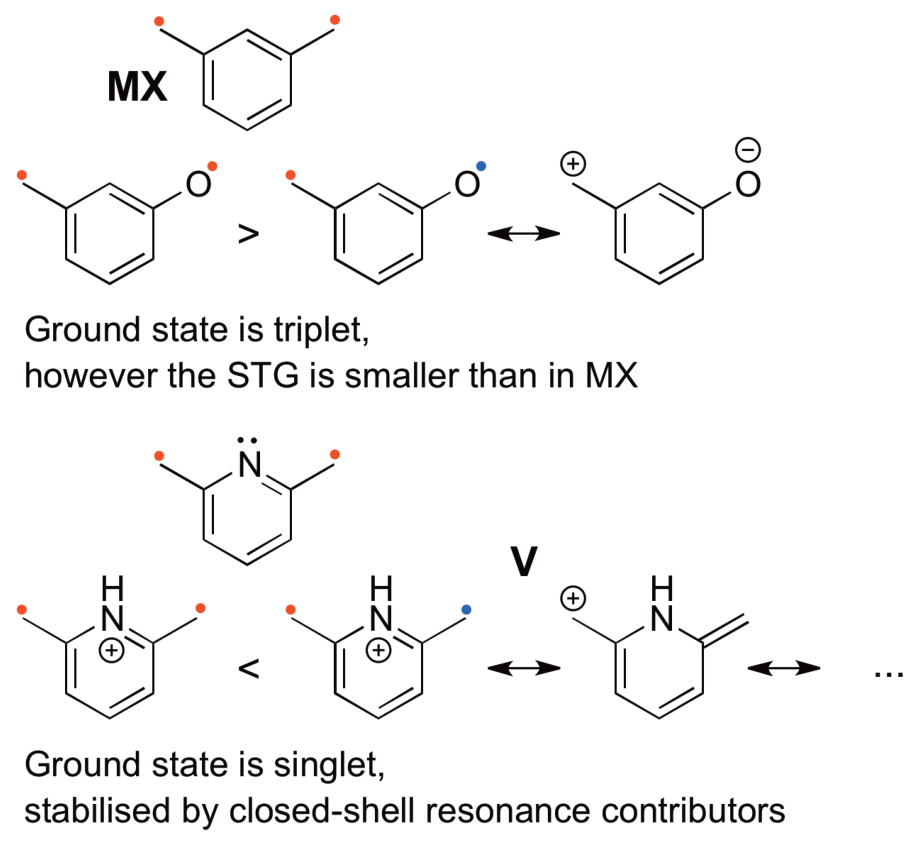
\includegraphics[width=0.95\linewidth]{fig06_ionic_resonance_spin_reversal.png}
    \column{0.47\textwidth}
    \begin{paperclaim}
      ``In the pyridinium analog of MX (V in Figure 6) this contribution exceeds the exchange and Coulomb terms,
      which formally favor the triplet state of this system with nondisjoint NBMOs.''
    \end{paperclaim}
    \onslide<2->{\small low-lying zwitterionic structures = small effective $U-V$\\
      $\Rightarrow$ $4t^2/(U-V)$ grows past $2k$ \;$\Rightarrow$\; singlet}
    \vskip0.2cm
    \onslide<3->{\small\cmuted{(a qualitative mapping: the review gives no numbers)}}
  \end{columns}
\end{frame}

\begin{frame}{Delocalised and localised: two views of one state}
  {\large
  \[
    a,b=\tfrac1{\sqrt2}(l\pm r)\quad\Rightarrow\quad
    a(1)a(2)-b(1)b(2)=l(1)r(2)+r(1)l(2)
  \]}
  \vskip0.2cm
  \begin{columns}[c]
    \column{0.48\textwidth}
    \begin{plainpanel}
      \centering\cgold{delocalised view}\\[2pt]
      two closed-shell configurations of equal weight: ``static correlation''
    \end{plainpanel}
    \column{0.48\textwidth}
    \onslide<2->{
    \begin{plainpanel}
      \centering\cgold{localised view}\\[2pt]
      one covalent configuration, no ionic part: ``no ionic character''
    \end{plainpanel}}
  \end{columns}
  \vskip0.3cm
  \onslide<3->{\centering\small same physics, different bookkeeping; the paper's two pictures are compatible\par}
\end{frame}
